\documentclass{article}
\usepackage{tikz}
\usetikzlibrary{positioning}

\begin{document}

\begin{figure}[h]
    % \centering
\hspace*{-2.8cm} % Adjust the value as needed
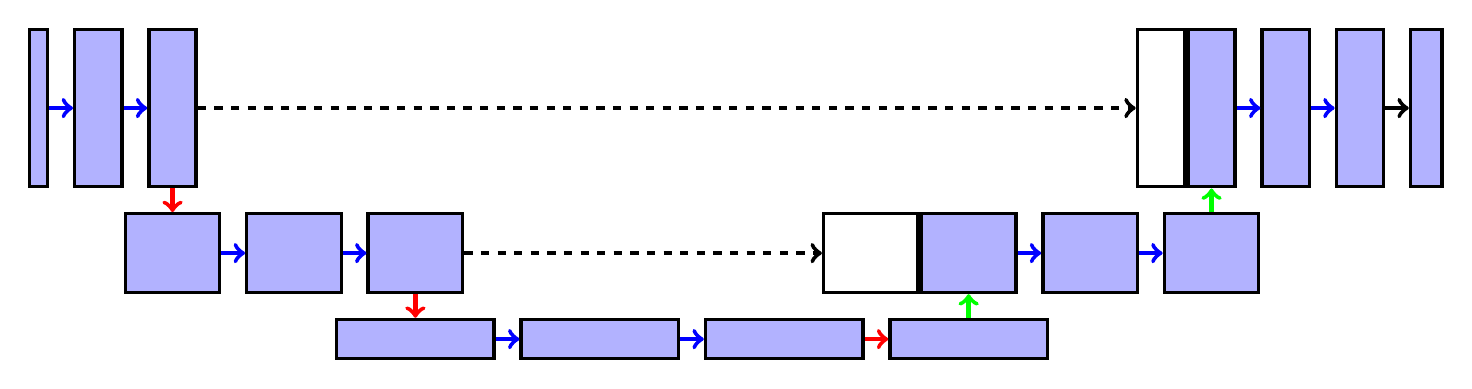
\begin{tikzpicture}[node distance=0.3cm, auto, very thick, transform shape, shift={(-10cm,0)}]
    % Define styles
    \tikzstyle{rec16_1} = [draw, rectangle, minimum width=0.1cm, minimum height=2cm, fill=blue!30]
    \tikzstyle{rec16} = [draw, rectangle, minimum width=0.6cm, minimum height=2cm, fill=blue!30]
    \tikzstyle{rec32} = [draw, rectangle, minimum width=1.2cm, minimum height=1cm, fill=blue!30]
    \tikzstyle{rec64} = [draw, rectangle, minimum width=2.0cm, minimum height=0.5cm, fill=blue!30]
    \tikzstyle{rec64_2} = [draw, rectangle, minimum width=2.0cm, minimum height=0.5cm, fill=blue!30]
    \tikzstyle{rec2} = [draw, rectangle, minimum width=0.4cm, minimum height=2cm, fill=blue!30]
    \tikzstyle{rec_white32} = [draw, rectangle, minimum width=1.2cm, minimum height=1cm, fill=white]
    \tikzstyle{rec_white16} = [draw, rectangle, minimum width=0.6cm, minimum height=2cm, fill=white]
    \tikzstyle{normalconv} = [->, ultra thick, blue]
    \tikzstyle{maxpool} = [->, ultra thick, red]
    \tikzstyle{upconv} = [->, ultra thick, green]
    \tikzstyle{finalconv} = [->, ultra thick, black]

    % ENCODER
    \node (en1_input) [rec16_1] {};
    \node (en1con1_output) [rec16, right=of en1_input] {};
    \node (en1con2_output) [rec16, right=of en1con1_output] {};

    \node (en2_input) [rec32, below=of en1con2_output] {};
    \node (en2con1_output) [rec32, right=of en2_input] {};
    \node (en2con2_output) [rec32, right=of en2con1_output] {};

    \node (en3_input) [rec64, below=of en2con2_output] {};
    \node (en3con1_output) [rec64, right=of en3_input] {};
    \node (en3con2_output) [rec64, right=of en3con1_output] {};
    \node (upcon1_input) [rec64_2, right=of en3con2_output] {};

    % DECODER
    \node (de1_input) [rec32, above=of upcon1_input] {};
    \node (skip1_output) [rec_white32, left=0cm of de1_input] {};
    \node (de1con1_output) [rec32, right=of de1_input] {};
    \node (de1con2_output) [rec32, right=of de1con1_output] {};

    \node (de2_input) [rec16, above=of de1con2_output] {};
    \node (skip2_output) [rec_white16, left=0cm of de2_input] {};
    \node (de2con1_output) [rec16, right=of de2_input] {};
    \node (de2con2_output) [rec16, right=of de2con1_output] {};

    % Final output layer
    \node (final_output) [rec2, right=of de2con2_output] {};

    % CONNECTIONS
    \draw[normalconv] (en1_input) -- (en1con1_output);
    \draw[normalconv] (en1con1_output) -- (en1con2_output);
    % \draw[maxpool] (en1con2_output) -- ++(0,-0.5) -| (en2_input);
    \draw[maxpool] (en1con2_output) -- (en2_input);
    
    \draw[normalconv] (en2_input) -- (en2con1_output);
    \draw[normalconv] (en2con1_output) -- (en2con2_output);
    % \draw[maxpool] (en2con2_output) -- ++(0,-0.5) -| (en3_input);
    \draw[maxpool] (en2con2_output) -- (en3_input);
    
    \draw[normalconv] (en3_input) -- (en3con1_output);
    \draw[normalconv] (en3con1_output) -- (en3con2_output);
    \draw[maxpool] (en3con2_output) -- (upcon1_input);
    
    % \draw[upconv] (en3con2_output) -- ++(0,0.5) -| (de1_input);
    \draw[upconv] (upcon1_input) -- (de1_input);
    \draw[normalconv] (de1_input) -- (de1con1_output);
    \draw[normalconv] (de1con1_output) -- (de1con2_output);
    
    % \draw[upconv] (de1con2_output) -- ++(0,0.5) -| (de2_input);
    \draw[upconv] (de1con2_output) -- (de2_input);
    \draw[normalconv] (de2_input) -- (de2con1_output);
    \draw[normalconv] (de2con1_output) -- (de2con2_output);
    
    \draw[finalconv] (de2con2_output) -- (final_output);

    % Skip connections
    \draw[->, dashed, ultra thick] (en2con2_output.east) -- ++(0.5,0) |- (skip1_output.west);
    \draw[->, dashed, ultra thick] (en1con2_output.east) -- ++(0.5,0) |- (skip2_output.west);

\end{tikzpicture}
\caption{U-Net Architecture Schematic Diagram}
\label{fig:my_unet}
\end{figure}

\end{document}
